\documentclass{article}

\usepackage{arxiv}

\usepackage[utf8]{inputenc}
\usepackage[T1]{fontenc}
\usepackage{amsmath,amsfonts}
\usepackage{nicefrac}
\usepackage{microtype}
\usepackage{graphicx}
\usepackage{booktabs}
\usepackage{tabularx}
\usepackage{multirow}
\usepackage{xcolor}
\usepackage{listings}
\usepackage{xspace}
\usepackage{url}
\usepackage{natbib}
\usepackage{hyperref}
\usepackage{cleveref}   %
\usepackage{doi}
\usepackage[section]{placeins}  %
\usepackage{float}                %
\raggedbottom                      %

\graphicspath{{figures/}}

\newcommand{\AFtwo}{AlphaFold2\xspace}
\newcommand{\AFthree}{AlphaFold3\xspace}

\newcommand{\TODO}[1]{\textcolor{red}{\textbf{[TODO: #1]}}}
\newcommand{\REF}[1]{\textcolor{blue}{\textbf{[REF: #1]}}}

\lstset{
  language=Python,
  basicstyle=\ttfamily\footnotesize,
  keywordstyle=\bfseries,
  commentstyle=\itshape\color{gray},
  stringstyle=\color{teal},
  numbers=left,
  numberstyle=\tiny\color{gray},
  frame=tb,
  breaklines=true,
  showstringspaces=false,
  captionpos=b
}

\title{Accelerator Choice Is Not Enough:\\
AlphaFold2 Inference on Cloud TPUs}

\date{September 28, 2026}

\author{
  Lorenzo Pazienza\thanks{Work carried out during the Stanford Summer
  Session 2026, using TPU~v5e infrastructure provided by Stanford
  University.} \\
  LUISS Guido Carli University \\
  Rome, Italy \\
  \texttt{lorenzo.pazienza@gmail.com} \\
  \And
  Ihab El Bani \\
  Al Akhawayn University \\
  Ifrane, Morocco \\
  \texttt{elbani.ihab@gmail.com} \\
}

\renewcommand{\headeright}{Preprint}
\renewcommand{\undertitle}{Preprint}
\renewcommand{\shorttitle}{AlphaFold2 Inference on Cloud TPUs}

\hypersetup{
  colorlinks=true, linkcolor=blue!50!black, citecolor=blue!50!black, urlcolor=blue!50!black,
  pdftitle={Accelerator Choice Is Not Enough: AlphaFold2 Inference on Cloud TPUs},
  pdfauthor={Lorenzo Pazienza, Ihab El Bani},
  pdfkeywords={TPU, JAX, XLA, automatic sharding, AlphaFold2, AlphaFold3, benchmarking},
}

\begin{document}
\maketitle

\begin{abstract}
AlphaFold2 is written in JAX, so the same inference code compiles and
runs unchanged on CPUs, GPUs and Google Cloud TPUs. That portability
makes the accelerator look like the main decision a user has to make.
We show that it is not. Running one AlphaFold2 inference workload
across a Colab CPU runtime, an NVIDIA T4 GPU and a dedicated eight-chip
Cloud TPU~v5e slice, we find a large hardware advantage for the TPU,
0.47\,s per call in steady state on a single chip against 13.1\,s on
the T4 in the same measurement campaign, and three ways in which the
software layer decides how much of it a user actually gets. The default
execution path uses one chip of the eight, and at list prices the idle
capacity makes the slice cost about as much per prediction as the GPU.
Batching with \texttt{jax.vmap} never exceeds single-query throughput,
while mapping queries across chips with \texttt{jax.pmap} gives eight
chips 6.5--7.9$\times$ the throughput of one on a matched grid;
automatic sharding leaves the per-chip footprint unchanged, consistent
with replication, most plausibly because AlphaFold2 carries no sharding
annotations. Our retained trace analysis of a first call at a new input
shape reports about three quarters of the traced span in JAX tracing
and compilation rather than execution. Reruns five weeks later
reproduced neither cloud baseline, the GPU one off by roughly a factor
of two, so the hardware ratio above is specific to one campaign.
\end{abstract}

\keywords{Tensor Processing Units \and JAX/XLA \and Automatic sharding \and
Data parallelism \and Protein structure prediction \and Benchmarking}


\section{Introduction}\label{sec:introduction}

AlphaFold2 made accurate protein structure prediction routine
\citep{jumper2021alphafold}, and in doing so turned it into a computing
workload: large screening campaigns run inference on thousands of
sequences, and each prediction is a deep network evaluated on
specialized hardware. Its public implementation is written in JAX, which
compiles the same Python program through XLA for CPUs, GPUs and Google's
Tensor Processing Units (TPUs). On paper this makes the choice of
accelerator a matter of picking the fastest or cheapest device. In
practice, the performance a user obtains depends on more than the
device: on how the program is compiled, on how its computation is mapped
onto the chips that are allocated, and on how stable the underlying
cloud machine is from one session to the next. For this class of
scientific workload, the gap between what the hardware can deliver and
what a user running the model actually gets has received little
systematic attention.

This paper measures that gap. We run the same AlphaFold2 inference code
on the same input on three backends: a Colab CPU runtime, an NVIDIA T4
GPU, and a dedicated eight-chip Google Cloud TPU~v5e slice. We then ask
three questions: how the backends compare on a single call, where the
time goes when a call is first compiled, and what it takes to put all
the allocated chips to work.

The single-call comparison favors the TPU by a wide margin: in steady
state, one TPU chip completes an inference call in 0.47\,s, 27.8$\times$
faster than the T4 in our August baseline
(Section~\ref{sec:results-hardware}).
That comparison comes with three qualifications. It is the performance of
\emph{one} chip: in the default execution path, seven of the eight
allocated chips hold no data at all, so a user pays for a full slice and
uses an eighth of it, and at list prices this idle capacity makes the
TPU slice cost about the same per prediction as the T4 GPU on that same
August baseline (Section~\ref{sec:cost}). The first call on each new
input shape is dominated by work that precedes execution: in a profiler
trace of the first call, about three quarters of the traced
model-application span is self time in JAX's tracing and compilation
path (Section~\ref{sec:profiling}). For one-off jobs, this cold start
matters more than steady-state speed. Finally, the CPU and GPU
baselines did not reproduce across Colab sessions weeks apart: the CPU became roughly
1.6--1.7$\times$ slower and the GPU about twice as fast, for reasons we
could not identify. The GPU change bears directly on the TPU-over-GPU
ratio above, so we report every session rather than a single canonical
value (Section~\ref{sec:rh-variability}).

The idle chips are not recovered by the obvious fix. Vectorizing the
model over a batch of queries with \texttt{jax.vmap} does not help:
throughput never exceeds that of a single query and falls to roughly
three quarters of it at batch sizes 4 and 8 (0.73$\times$ and
0.74$\times$). Mapping independent queries
across devices with \texttt{jax.pmap} does put all eight chips to work:
on a matched grid, eight chips deliver 6.53$\times$ to 7.91$\times$ the
throughput of one, the efficiency rising with sequence length
(Section~\ref{sec:scaling}); against the single-query baseline, which
uses a different input family, the gain is 6.92$\times$.
JAX's automatic partitioner, which is meant to make such manual
mapping unnecessary, leaves the per-chip memory footprint of a
single-query run unchanged from the one-chip case, consistent with
replicating the model rather than splitting it. Our best explanation
is that the model carries no sharding annotations, leaving the
partitioner nothing from which to derive a split, which is the
documented fallback of an annotation-driven partitioner
\citep{xu2021gspmd,shardy2026} and matches the reported effect of
stripping sharding structure from such a system \citep{drjax2024}.
We did not retain the compiler evidence that would confirm it. AlphaFold2's own
ensembling cannot be split this way either, because the public
implementation runs ensemble members in a sequential \texttt{while\_loop}
rather than along an array axis. We build the ensemble outside the
model instead: eight differently seeded featurizations of
one query, one per chip under \texttt{pmap}, with their
\texttt{predicted\_lddt} logits averaged by \texttt{pmean}. AlphaFold2's
source and its internal \texttt{num\_ensemble\,=\,1} path are left
untouched, so this demonstrates that an ensemble can be spread across
the slice; it does not replace AlphaFold2's own ensembling
(Section~\ref{sec:parallelism}).

Prior work has optimized AlphaFold2 training and long-sequence
inference on GPU clusters through model parallelism (FastFold) and through pipeline separation with
compilation reuse (ParaFold) \citep{cheng2024fastfold,zhong2022parafold}.
Both target NVIDIA GPUs; neither reports TPU experiments.
Closer to the hardware, JAXBench includes operators extracted from
AlphaFold2 among its TPU kernel benchmarks \citep{jaxbench2026}, and a recent characterization of
AlphaFold3 profiles its bottlenecks on CPUs and GPUs
\citep{iiswc2025af3}; to our knowledge, neither measures end-to-end
AlphaFold2 inference on TPU.

Our contributions are:
\begin{itemize}
  \item a controlled comparison of AlphaFold2 inference on CPU, GPU and
    a multi-chip TPU slice, using identical code and input, with its
    provenance gaps and cross-session variability reported
    (Sections~\ref{sec:methodology} and~\ref{sec:results-hardware});
  \item a retained trace analysis of the cold-start regime on TPU,
    reporting that about three quarters of the traced \texttt{apply\_fn}
    span is JAX tracing and compilation rather than execution, consistent
    with the compilation cost that ParaFold identified on GPU,
    together with a profiler-overhead correction to our CPU and GPU
    first-call timings, which we could not verify on TPU
    (Section~\ref{sec:profiling});
  \item a measurement showing that vectorization does not raise
    throughput for this model while explicit data parallelism across
    chips does (Section~\ref{sec:parallelism});
  \item an observation that automatic sharding leaves AlphaFold2's
    per-chip footprint unchanged, with a hypothesis for why, and a
    demonstration that an
    ensemble can instead be built outside the model and mapped across
    chips, leaving the model source untouched
    (Section~\ref{sec:parallelism});
  \item a matched 16-point grid over chip count and sequence length,
    with measured eight-over-one-chip speedups of 6.53--7.91$\times$, a
    descriptive fit to it, and its consequences for cost per prediction
    (Sections~\ref{sec:scaling} and~\ref{sec:cost});
  \item a portability finding across model generations: the
    AlphaFold3 release we tested accepts only CPU, GPU and Apple MPS
    backends, not TPU (Section~\ref{sec:alphafold3}).
\end{itemize}

Section~\ref{sec:background} introduces TPUs, the JAX/XLA compilation
model and the computational structure of AlphaFold2.
Section~\ref{sec:methodology} describes the setup, and
Sections~\ref{sec:results-hardware} to~\ref{sec:alphafold3} present the
results. Section~\ref{sec:related-work} places them in context,
Section~\ref{sec:discussion} discusses what they imply for users of
scientific JAX workloads, and Sections~\ref{sec:limitations}
and~\ref{sec:conclusion} state the limitations and conclude.


\section{Background}\label{sec:background}

\subsection{TPU slices and device placement}
\label{sec:bg-tpu}

A single Cloud TPU v5e chip, the generation used throughout this
work, provides 197\,bf16 TFLOPs and 16\,GB of HBM with a memory bandwidth of 800\,GiB/s
\citep{googletpuv5e}. Multiple chips on a slice are connected by a
dedicated Inter-Chip Interconnect (ICI) fabric arranged as a 2D torus,
independent of the host network, allowing up to 256 chips per pod to
exchange activations and gradients without going through the datacenter
network \citep{googletpuv5e}. Because v5e has no dedicated
peer-reviewed architecture paper, we cite the vendor documentation for
per-chip specifications and the two Jouppi ISCA papers
\citep{jouppi2017tpu, jouppi2023tpuv4} for the systolic-array design and
its evolution across TPU generations.

Software sees each chip as an explicit JAX device. Nothing about the
torus interconnect is used unless the program says so. A slice with
$n$ chips visible does not automatically distribute an $n$-chip job
across them: how work is mapped onto devices is decided by the JAX/XLA
compilation layer, or explicitly by the programmer, not by the
hardware. Section~\ref{sec:parallelism} measures what that layer does
with AlphaFold2 on this slice.

\subsection{The JAX/XLA compilation model}
\label{sec:bg-jax}

JAX traces Python functions into an intermediate representation
(a \texttt{jaxpr}) the first time they are called with a new
combination of argument shapes, then lowers that representation to
XLA HLO and compiles it to a binary for the target device. The
profile labels the function that performs this trace-and-compile step
\texttt{cache\_miss}, after the fallback path taken when JAX's
fast-path jit cache does not hold an entry for the call; for a
Haiku-based model such as AlphaFold2, this trace walks through
Haiku's \texttt{apply\_fn}, lowering the full Evoformer computation
graph into XLA's representation before a single matrix multiply has
executed. Compilation is keyed on input shapes and dtypes, together
with any static arguments: a function called again with the same
signature reuses the compiled binary, while a change to it (a different
sequence length, or a switch between \texttt{float32} and
\texttt{bfloat16}) triggers a fresh trace and compile. A workload's
\emph{first} call at a given input shape is therefore different work
from every call after it, and the timing methodology has to separate
the two (Section~\ref{sec:methodology}). A persistent compilation
cache can carry compiled binaries across process restarts, avoiding
the XLA-compile step on a shape that has already been compiled once,
but a fresh process still has to re-trace the Python program down to a
jaxpr before it can consult that cache, so a persistent cache reduces
cold-start cost without eliminating it.

JAX's own transformations for expressing
parallelism, \texttt{vmap} for vectorizing a function over a batch axis
and \texttt{pmap} for mapping a function across physical devices with
an explicit per-device argument axis, are different operations even
though both add a leading axis to a function's inputs: \texttt{vmap}
changes what a single device computes, \texttt{pmap} changes which
device computes it. XLA's automatic partitioner, in turn, can shard a
computation across devices
without a user manually writing per-device code, but it does so by
propagating sharding decisions outward from explicit annotations,
principally \texttt{PartitionSpec} constraints placed on inputs,
outputs or intermediates. (JAX also offers \texttt{shard\_map}, the
manual complement to automatic partitioning: there the programmer
writes the per-device code and the collectives.) A computation carrying no annotations gives the partitioner
nothing to propagate from, and its documented fallback is to replicate
the computation rather than split it.

\subsection{AlphaFold2's computational structure}
\label{sec:background-af2}

AlphaFold2 predicts a protein's three-dimensional structure from its
amino-acid sequence by iterating two representations against each
other: a multiple sequence alignment (MSA) representation, one row per
homologous sequence, and a pair representation, one entry per pair of
residues, encoding the model's evolving belief about which residues
are close in space. The Evoformer block updates both representations
through attention operations (including triangular self-attention and
triangular multiplicative updates on the pair representation, whose
cost scales with the number of residues beyond simple quadratic
attention) before a structure module converts the final single and pair
representations into three-dimensional coordinates
\citep{jumper2021alphafold}. The whole Evoformer-plus-structure-module
pipeline is then \emph{recycled}: its own output is fed back as input
for a further pass, refining the prediction over a small, fixed number
of iterations \citep{jumper2021alphafold}. AlphaFold2's public
implementation is written in JAX and Haiku, which is what makes it
usable, unmodified, as a systems benchmark across JAX-supported
backends (Section~\ref{sec:methodology}): a real, widely used model
with an attention-heavy graph and small sequential control flow.
Its diffusion-based successor,
AlphaFold3, replaces the Evoformer/structure-module pair with a
different architecture, and its released entry point accepts a
different set of backends (Section~\ref{sec:alphafold3}). We report
those as two separate facts: nothing we measured connects the one to
the other.

One further structural detail matters for multi-chip execution.
AlphaFold2 can run an \emph{ensemble}: several stochastic variations of
the same input are processed and their representations averaged. The
released configuration uses a single member for evaluation, as do our
runs. When more members are requested, the public implementation does
not compute them along an array axis. It iterates over them with a
sequential \texttt{hk.while\_loop} inside \texttt{AlphaFoldIteration},
and recycling is implemented as a \texttt{while\_loop} in the same way.
Sequential control flow of this kind offers no tensor dimension to
split across devices, so the ensemble cannot be parallelized by
sharding its arrays; spreading members across chips requires mapping
them explicitly, which is what we do in Section~\ref{sec:parallelism}.
This is a separate matter from the partitioner behavior we observe on a
single-member forward pass, for which the most plausible explanation
is the general mechanism described in Section~\ref{sec:bg-jax}: the
model carries no sharding annotations for the partitioner to propagate.
Section~\ref{sec:parallelism} states what evidence we have for that
and what we lack.


\section{Methodology}\label{sec:methodology}

This section describes the hardware, software, workload and timing
procedure behind every measurement in the paper, and states what our
records do not contain. The full provenance audit, with a
file-level source for each statement below, is part of the released
repository (see Code and Data Availability).

\subsection{Hardware}
\label{sec:meth-hardware}

We compare three backends running the same AlphaFold2 inference code
(Table~\ref{tab:meth-hardware}). CPU and GPU runs used Google Colab
runtimes; TPU runs used a Google Kubernetes Engine cluster in
\texttt{us-west4} provided through Stanford's ME344 course.

\begin{table}[H]
\centering\small
\caption{Hardware and software per backend. ``Not recorded'' means our
run artifacts do not contain the value; these gaps are discussed in
Section~\ref{sec:limitations}.}
\label{tab:meth-hardware}
\begin{tabularx}{\linewidth}{>{\raggedright\arraybackslash}p{0.17\linewidth}>{\raggedright\arraybackslash}X>{\raggedright\arraybackslash}X>{\raggedright\arraybackslash}X}
\toprule
 & CPU (Colab) & GPU (Colab) & TPU (GKE) \\
\midrule
Device & x86\_64 CPU runtime, 2 vCPU (from our write-up, not a
recorded field in the run artifacts); August host CPU model not
recorded; September reruns: Intel Xeon @ 2.20\,GHz (family 6,
model 79) & NVIDIA Tesla T4, 15{,}360\,MiB, compute capability 7.5,
driver 580.82.07 & TPU v5e slice (\texttt{tpu-v5-lite-podslice},
topology 2$\times$4): 8 chips, 16.9\,GB HBM limit per chip \\
Host CPU / RAM & same as device & not recorded (August) & not recorded \\
JAX & unpinned in August (resolved version not recorded); 0.10.2 in
the September reruns & unpinned, \texttt{jax[cuda12]} (resolved
version not recorded) & \texttt{jax[tpu]==0.10.2} \\
Scheduling & interactive notebook & interactive notebook & Kubernetes
Job, Kueue queue, 8 chips requested \\
\bottomrule
\end{tabularx}
\end{table}

Two properties of this setup bear on the results. The TPU allocation
is always the full 8-chip slice, but in the default single-query
execution path only one chip performs work: seven of the eight chips
report zero bytes of device memory in use. Single-query TPU timings
therefore measure one v5e chip (Section~\ref{sec:rh-onechip}), while
cost is billed for all eight (Section~\ref{sec:cost}). The backends are
also not equally isolated: the TPU ran as a dedicated Kubernetes
Job, whereas the CPU and GPU ran on shared Colab runtimes whose
underlying machine is chosen by the provider and may change between
sessions. Section~\ref{sec:rh-variability} reports how repeated CPU and
GPU timings varied across sessions; we did not isolate a cause, and
shared tenancy remains a hypothesis there rather than a demonstrated
one.

\subsection{Software}
\label{sec:meth-software}

All AlphaFold2 runs use the public DeepMind implementation, cloned from
its default branch at run time. The August runs did not record which
commit that resolved to; the September reruns do, in their environment
files. The AlphaFold2 source is not modified. One compatibility shim
is applied from outside it: our scripts wrap \texttt{jax.numpy.clip} so
that the \texttt{a\_min}/\texttt{a\_max} keyword arguments used by
AlphaFold2 map onto the argument names of current JAX releases. No
container image digest or lockfile was used for the original runs: TPU
Jobs started from a floating \texttt{python:3.12-slim} image and
installed packages at start-up, with only JAX pinned, and the Colab
notebooks installed JAX and AlphaFold2's dependencies unpinned. For the
September reruns, each result is stored together with the benchmark
repository commit it was run from and a capture of the environment
(installed package versions and host CPU).

\subsection{Workload}
\label{sec:meth-workload}

Every AlphaFold2 run uses the \texttt{model\_3} configuration (no
templates), a single ensemble member, no recycling
(\texttt{num\_recycle}~$=0$) and float32 precision, unless an experiment
varies one of these explicitly (the recycling, precision and
model-comparison sweeps).

\paragraph{Input sequences.} Single-query experiments fold a fixed
synthetic 118-residue sequence. The sequence-length sweep, the
\texttt{vmap} batching experiment, the multi-query \texttt{pmap}
experiment and the chip-count scaling grid instead use the 20-letter
amino-acid alphabet repeated to the target length (rotated per batch
item), including at 118 residues. These two input families are
therefore not identical. The one place the paper sets a number from
each family side by side is the 6.92$\times$ multi-query throughput
gain of Section~\ref{sec:parallelism}, whose denominator is the
fixed-sequence single-query baseline; we flag that mismatch where the
figure appears, and treat the matched chip-count grid as the cleaner
comparison.

\paragraph{MSA and features.} To isolate model execution from the data
pipeline, no genetic database search is run and no templates are used:
the MSA contains only the query sequence, built with AlphaFold2's own
parsing and feature code. Feature processing happens before any timer
starts. The trivial MSA does not shrink the compiled graph, because
AlphaFold2 pads its MSA tensors to fixed sizes: the logged model inputs
are \texttt{msa\_feat} of shape $(1, 512, 118, 49)$ and
\texttt{extra\_msa} of shape $(1, 5120, 118)$. All feature, parameter
and prediction seeds are fixed to 0, with one exception: the external
ensemble experiment of Section~\ref{sec:parallelism} builds its eight
feature sets with seeds 0--7, since identical seeds would give
identical members. Parameter initialization and the shared model PRNG
stay at 0 there too.

\paragraph{Why random weights.} AlphaFold2 is run with randomly
initialized parameters; the trained checkpoint is never loaded. This is a
systems study: the question is where time goes during compilation and
execution, not how accurate the predicted structures are, and the
compiled graph's shapes and operations do not depend on parameter
values. The predicted structures are therefore meaningless and are
never interpreted, and timing equivalence with trained weights is
argued rather than measured: we did not time a run with trained
weights, so value-dependent runtime effects cannot be ruled out.
The AlphaFold3 runs (Section~\ref{sec:alphafold3}) use the real, trained
AlphaFold3 weights.

\subsection{Timing procedure}
\label{sec:meth-timing}

All times are host wall-clock (\texttt{time.time()}). Every timed
\texttt{predict} call is followed by \texttt{jax.block\_until\_ready},
so that asynchronous accelerator work is included; the
\texttt{init\_params} timer has no such explicit barrier, so any device
work it leaves outstanding is not counted in that region. Each single-query process
times three consecutive regions: parameter initialization
(\texttt{init\_params}, including its own tracing and compilation), a
first \texttt{predict} call, which compiles and executes the model, and
a second, identical \texttt{predict} call, which reuses the compiled
program and is reported as the \emph{steady state}. The first call is
the only warm-up. The timed \texttt{predict} region also includes the
confidence metrics that AlphaFold2 computes on the host after the
forward pass.

\paragraph{Repeated steady-state calls.} In the original August
baselines, the steady state is a single call per process. For the
September CPU and GPU reruns, the committed script repeats the
steady-state call a configurable number of times and makes the profiler
optional: each rerun times five consecutive steady-state calls in the
same process, with the profiler disabled, and we report their mean and
sample standard deviation.

\paragraph{Profiler overhead on the first call.} In the August and TPU
runs of the single-query and \texttt{vmap} scripts, the first
\texttt{predict} runs inside a
\texttt{jax.profiler.trace} context, and closing that context is inside
the timer. The Colab logs let us measure this directly: after
\texttt{predict} returned, the timer kept running for another 36.00\,s
on CPU and 42.02\,s on GPU, while the same \texttt{block\_until\_ready}
took under a millisecond on the second call. Reported first-call times
from these scripts therefore include trace finalization; steady-state
times are unaffected. Section~\ref{sec:rh-coldstart} reports cold-start
ratios corrected for this overhead on CPU and GPU. No TPU run log
survives, so the size of the overhead on TPU is unknown. The
\texttt{pmap}, ensemble-sharding and auto-mesh scripts do not use the
profiler, so their first-call times are not comparable with those of
the single-query script.

\paragraph{Multi-chip experiments.} The multi-query \texttt{pmap} and
\texttt{vmap} experiments report throughput as batch size divided by the
steady-state call time. Device memory is read once per process from
JAX's per-device memory statistics after the second call; the reported
peak is the process-lifetime peak.

\paragraph{AlphaFold3.} AlphaFold3 is timed from its own log: model
inference for one seed and five diffusion samples, which includes JIT
compilation because AlphaFold3 makes a single model call per process
with no warm-up. Because recycling depth, compilation and sample
accounting all differ between the two models, we report no
AlphaFold3-to-AlphaFold2 speed ratio (Section~\ref{sec:alphafold3}).

\subsection{Repetitions and noise}
\label{sec:meth-repetitions}

Most experiments are a single process per configuration point. The
auto-mesh partitioning experiment was run twice, with steady states of
0.472\,s and 0.473\,s, but the only
deliberate \emph{noise characterization} on the TPU ran the
single-query benchmark three
times in the same pod, with a coefficient of variation of 0.12\% on
steady state, 0.82\% on \texttt{init\_params} and 1.00\% on the first
call. This noise estimate applies to the TPU setup only. Access to the
TPU cluster ended with the course, so the TPU measurements cannot be
repeated. For the shared Colab runtimes, we instead reran the CPU
baseline in three further sessions (2026-09-15, -16 and -17) and the GPU
baseline in one (2026-09-15), five steady-state calls each
(Section~\ref{sec:rh-variability}). Experiments that share a Kubernetes
Job ran back to back in one pod, in a fixed order.

\subsection{Provenance}
\label{sec:meth-provenance}

The original results were committed together with the benchmark scripts
in a single commit, so version control cannot tie a result to the
script revision that produced it. The August CPU and GPU baselines were
produced by an uncommitted copy of the script embedded in the Colab
notebooks, with the same timing structure as the committed version; the
TPU baseline result matches neither surviving script version. TPU run
dates were not recorded. Version control only bounds them from above,
since all TPU results were already committed by 2026-08-11 (most of them
on 2026-08-08). The September
reruns close this gap for CPU and GPU, since each is tied to an explicit
commit and a captured environment.

The consequence is that the August baseline runs, and the headline
ratios computed from them, cannot be regenerated from the repository
as it stands. We know what was measured and from which
result file each number comes, because the catalogue records that. What
we cannot do is re-execute the exact configuration that produced them.
The September reruns are reproducible in that stronger sense, and the
comparison between the two is reported in
Section~\ref{sec:rh-variability}. Everything else our records do not
contain is listed with its consequences in Section~\ref{sec:limitations}.



\section{Single-Chip Hardware Comparison}\label{sec:results-hardware}

\subsection{Main comparison}
\label{sec:rh-main}

Table~\ref{tab:rh-main} reports \texttt{init\_params}, first
\texttt{predict} and steady-state timing for the same AlphaFold2
forward pass (\texttt{model\_3}, 118 residues, \texttt{num\_recycle=0},
float32, untrained weights) on CPU (Google Colab), GPU (NVIDIA T4,
Google Colab) and TPU (a single v5e chip on the Stanford cluster
slice). These are the original August 2026 baseline runs, each a single
call with no repetition. None of the three result
files records a timestamp or a session identifier. Archived
execution output in the August notebooks dates the CPU and GPU runs
to 2026-08-08 by the notebook's own clock; the TPU run is bounded only
by the commit that carries it. Nothing establishes that the three
backends ran within one session
(Section~\ref{sec:meth-provenance}); Section~\ref{sec:rh-variability}
reports what changed when we reran two of the three backends five
weeks later.

\begin{table}[H]
\centering\small
\caption{The August 2026 single-call baseline on the three backends:
one 118-residue inference per backend, untrained weights, float32. The
TPU row is a single v5e chip.}
\label{tab:rh-main}
\begin{tabular}{lrrr}
\toprule
Backend & \texttt{init\_params} (s) & First \texttt{predict} (s) & Steady state (s) \\
\midrule
CPU        & 41.99  & 271.98 & 212.113 \\
GPU (T4)   & 109.16 & 97.62  & 13.086  \\
TPU (v5e)  & 36.6   & 27.78  & 0.47    \\
\bottomrule
\end{tabular}
\end{table}

At steady state, the TPU is 451$\times$ faster than the CPU and
27.8$\times$ faster than the T4; the T4 itself is 16.2$\times$ faster
than the CPU. Each ratio compares exactly two measured points. We do
not chain any two of them into a claim about the TPU's advantage over
the CPU \emph{through} the GPU.
Figure~\ref{fig:rh-speedup} shows the same three timings on a log
scale, with each backend's speedup over the CPU; the TPU row carries
the single-chip caveat of Section~\ref{sec:rh-onechip}.

\subsection{TPU figures are single-chip figures}
\label{sec:rh-onechip}

The Stanford cluster slice exposes 8 TPU chips, but the single-query
path used for every number in Table~\ref{tab:rh-main} places work on
only one of them: the other seven report 0\,MB of device memory in
use throughout the run. The TPU numbers above therefore compare one
v5e chip against one T4 GPU or a two-vCPU Colab runtime (the vCPU
count is from our write-up, not a recorded field), not an 8-chip slice against
a single device. This caveat applies wherever these ratios are
cited later in the paper, including the central claim in
Section~\ref{sec:introduction}. Section~\ref{sec:parallelism} is about
what changes once the other seven chips are put to work.

\begin{figure}[H]
  \centering
  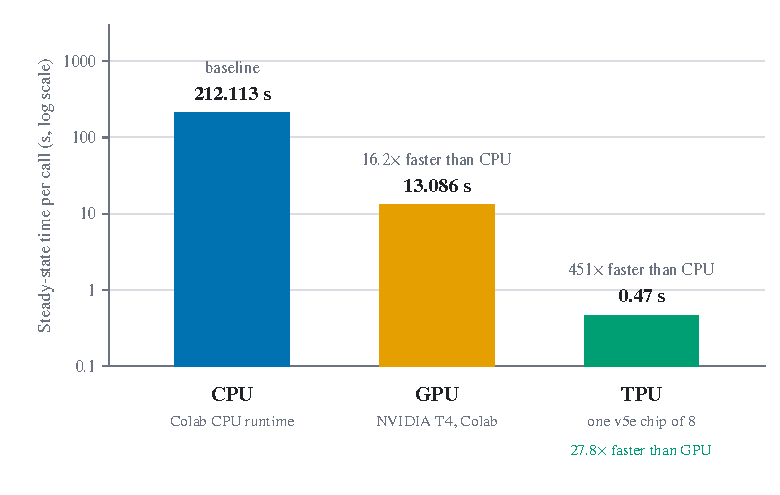
\includegraphics[width=0.75\linewidth]{speedup_hardware.pdf}
  \caption{Steady-state time per AlphaFold2 inference call (log scale),
  with the speedup of each backend over the CPU. The TPU value uses one of the slice's eight chips
  (Section~\ref{sec:rh-onechip}). All values are single-call August
  2026 baselines; Section~\ref{sec:rh-variability} reports how CPU and
  GPU timings changed across sessions.}
  \label{fig:rh-speedup}
\end{figure}

\subsection{The cold-start regime, corrected for profiler overhead}
\label{sec:rh-coldstart}

The first \texttt{predict} call is far more expensive than steady
state (271.98\,s vs.\ 212.113\,s for CPU, 97.62\,s vs.\ 13.086\,s for
GPU) because it includes JIT compilation of the full computation
graph (Section~\ref{sec:background}), not just execution. Read at face
value this gives cold/steady ratios of 1.28$\times$ (CPU) and
7.46$\times$ (GPU). Both first-\texttt{predict} timings, however, were
captured with \texttt{jax.profiler.trace} running inside the timed
region, and trace finalization itself measurably inflates the timer:
36.00\,s on CPU and 42.02\,s on GPU
(Section~\ref{sec:profiling}). Subtracting that overhead gives
corrected cold/steady ratios of approximately 1.11$\times$ for CPU and
4.25$\times$ for GPU: the compilation cost is real, but roughly
40\% smaller than the raw numbers suggest for GPU, and close to
negligible for CPU. The equivalent TPU correction cannot be applied:
no TPU run log recording profiler overhead separately is in the
repository, so the TPU's raw 59.1$\times$ cold/steady ratio is neither
confirmed nor corrected, and we do not report a corrected TPU figure.

\subsection{Cross-session variability, on two backends}
\label{sec:rh-variability}

Two of the three backends were rerun five weeks later, on
2026-09-15, with the same input and the same metric definitions as the
August baseline, from a committed revision of the benchmark script (the
August runs used an uncommitted copy of the script, so code identity
with August cannot be verified); the CPU backend was rerun twice more,
on 2026-09-16 and 2026-09-17. No rerun matches the August baseline
(Figure~\ref{fig:rh-variability}).

The CPU steady state rose from 212.113\,s (n=1, August) to
$348.861 \pm 4.690$\,s (n=5, 2026-09-15), $351.891 \pm 4.303$\,s
(n=5, 2026-09-16) and $359.273 \pm 2.787$\,s (n=5, 2026-09-17). The
three September sessions span 3\% and all sit 1.64--1.69$\times$ above
the August value. All three ran on the same host CPU model (an Intel
Xeon at 2.20\,GHz, family 6, model 79) with the same JAX version
(0.10.2); for the August session neither the host CPU model nor the JAX
version was recorded, so the gap cannot be attributed to either. With
four session-level data points the pattern looks less like symmetric
noise around a stable mean and more like a level shift between August
and September; four sessions are not enough to say which of the two
levels is typical for this Colab tier. The GPU steady state moved the other direction, from
13.086\,s (n=1, August) to $6.567 \pm 0.057$\,s (n=5, 2026-09-15), an
almost 2$\times$ \emph{drop}; there is only one September data point for
this backend. In neither case does the repository record a verified cause:
for GPU specifically, both sessions report identical GPU model,
driver and compute capability; the script copy and the numpy version
differ, while the August session's JAX version and host CPU were never
recorded, so those cannot be compared at all. No rerun isolates any of
these as the source of the gap. We report all
session values rather than picking one as canonical.

\begin{figure}[H]
  \centering
  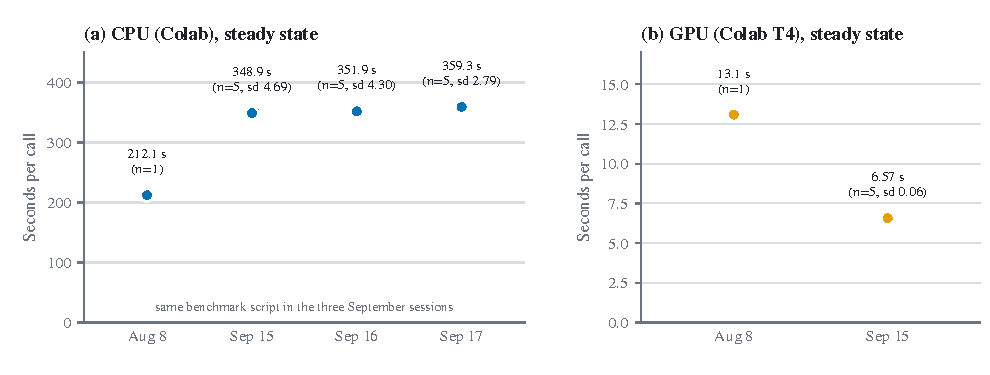
\includegraphics[width=\linewidth]{session_variability.pdf}
  \caption{Steady-state time per call across Colab sessions for the
  same benchmark and input. (a) CPU: the August baseline (one call) and
  three September sessions (five calls each, mean and sample standard
  deviation). (b) GPU (T4): the August baseline and one September
  session. Neither backend reproduced its August value; the two moved in
  opposite directions.}
  \label{fig:rh-variability}
\end{figure}

Prior reports of cloud benchmark instability put our gaps in context,
though they do not fully account for them. Surveying that literature,
\citet{bulej2020duet} report differences of around 15\% among
instances sharing a CPU type, and similar differences for one instance
over time, while differences as large as 280\% appear between
\emph{different} CPU types. Those figures are examples from particular
studies, not bounds, so they do not tell us which case our CPU gap
(August vs.\ the September sessions, 64--69\%) and GPU gap
(approximately 100\%) fall into. A host reassignment between sessions,
which the provider does not expose to the tenant, would be consistent
with both gaps; so would a change in
the resolved software environment, which the August runs did not
record. Neither can be confirmed: the September sessions record their
host CPU and package versions, the August ones do not, so no matched
comparison is possible.
What is unusual about
our case is not the magnitude but that it appears on two different
backends of the same benchmark, run weeks apart. The two are not
independent observations: both are Google Colab runtimes, sharing a
provider and a tenancy model, and the evidence behind them is thin:
one August call per backend, three September CPU sessions and one
September GPU session. We read this as consistent with a phenomenon
the cloud-systems literature already documents for general compute,
not as independent confirmation of it on ML accelerators
(Section~\ref{sec:limitations}). Every ratio in this paper that is
derived from the August GPU baseline (B-10, B-11 and B-14 in our
results catalogue, and with them the GPU cost figures C-06 and C-09 of
Section~\ref{sec:cost}) inherits this open gap, and we did not recompute them against
the September value.


\section{Profiling the Cold-Start Regime}\label{sec:profiling}

Section~\ref{sec:results-hardware} showed that the first call to
AlphaFold2's forward pass at a new input shape is far more expensive
than steady state, and that part of that cost is an artifact of
capturing the call inside a profiler trace rather than compilation
itself (Section~\ref{sec:rh-coldstart}). This section looks inside a single
first call to identify, at the function level, where the remaining
cost goes.

\subsection{Tracing a first call}
\label{sec:prof-method}

We captured one first-\texttt{predict} call for the single-query TPU
configuration (\texttt{model\_3}, 118 residues, \texttt{num\_recycle=0})
inside \texttt{jax.profiler.trace}, copied the resulting trace off the
pod before it was reclaimed, and inspected it in Chrome's trace
viewer. TPU pods on this cluster are torn down within roughly a
minute of job completion, so capturing the trace file required an
explicit copy step while the pod was still alive.

\subsection{The \texttt{cache\_miss} finding}
\label{sec:prof-cachemiss}

The traced call stack descends from AlphaFold2's outer
\texttt{apply\_fn} wrapper, which itself accounts for essentially none
of the traced time, into a function named \texttt{cache\_miss}, defined
in JAX's own \texttt{pjit.py}. Its purpose is to trace and compile a
computation the first time JAX encounters a given input shape. Of the
16.56\,s spanned by the traced \texttt{apply\_fn} call, 12.55\,s (about
76\%) is self time inside \texttt{cache\_miss} itself, not in any
function it calls. These trace figures come from the analysis written
up when the trace was taken; the raw profiler trace is not in the
repository, so they are reported figures that cannot be re-derived
from a retained artifact (Section~\ref{sec:limitations}).
Below \texttt{cache\_miss}, the call stack descends through
\texttt{\_infer\_params}, \texttt{\_trace\_for\_jit}, and
\texttt{trace\_to\_jaxpr} into Haiku's own \texttt{apply\_fn}, which
lowers AlphaFold2's Evoformer computation into XLA's intermediate
representation. Every frame in this path executes on the host. The
TPU device track in the same trace shows only a handful of brief
marks near the start of the window, and is otherwise idle for nearly
the full 16.56\,s while the host finishes tracing and compiling.

The 76\% figure is a share of the traced span, not of the
first-\texttt{predict} call as a whole: the trace covers 16.56\,s,
while the first-\texttt{predict} timings reported in
Section~\ref{sec:results-hardware} run 27.43--28.80\,s
in the runs that measure it directly. The two are separate captures
of related but not identical work, and the trace does not by itself
explain the gap between them. We report the 76\% figure only as a
property of the traced \texttt{apply\_fn} span: three quarters of that
span is JAX's own tracing-and-compilation machinery, concentrated in a
single named function, rather than TPU execution, data movement or
AlphaFold2's own arithmetic.

\begin{figure}[H]
  \centering
  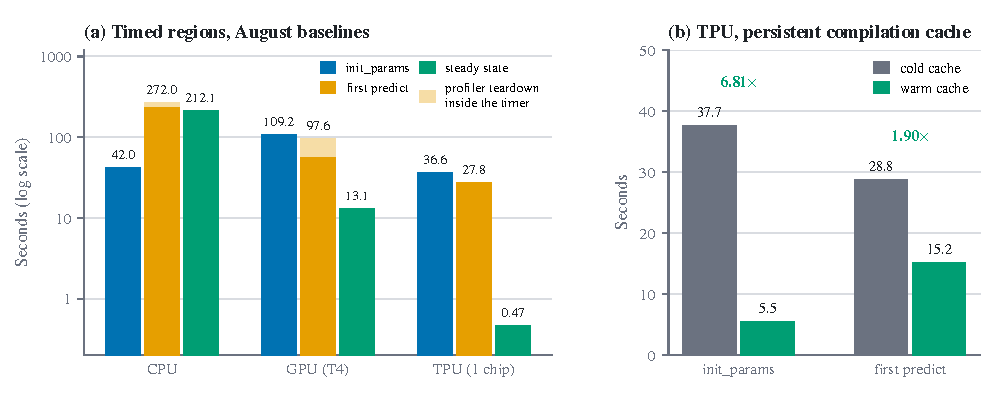
\includegraphics[width=\linewidth]{coldstart_regions.pdf}
  \caption{The cold-start regime. (a) The three timed regions of the
  August baselines on each backend, on a log scale. On CPU and GPU the
  lighter top segment of the first-\texttt{predict} bar is the profiler
  teardown that ran inside the timer (36.00\,s and 42.02\,s,
  Section~\ref{sec:rh-coldstart}); the TPU bar cannot be corrected
  because no TPU run log survives. (b) On TPU, a persistent compilation
  cache shortens \texttt{init\_params} 6.81$\times$ and the first
  \texttt{predict} call 1.90$\times$ in a fresh process; the steady state
  is unchanged.}
  \label{fig:coldstart}
\end{figure}

\subsection{Compilation cache}
\label{sec:prof-cache}

A persistent JAX compilation cache stores compiled XLA binaries across
process restarts, so a second process at the same input shape can skip
the compile step that produced them. Comparing a cold process against
one with a warm cache, on the same single-query configuration
(Figure~\ref{fig:coldstart}b),
\texttt{init\_params} drops from 37.68\,s to 5.53\,s, a 6.81$\times$
speedup, and the first \texttt{predict} call drops from 28.80\,s to
15.19\,s, a 1.90$\times$ speedup.
These are two different compilations and the two speedups should not
be compared to each other or to the 12.55\,s \texttt{cache\_miss}
figure above: the cache experiment and the trace are separate runs, and
a warm cache still requires a fresh process to re-trace the Python
program down to a jaxpr before it can consult the cache, which
plausibly accounts for part of the 15.19\,s that remains on the warm
first call. The comparison does establish that most of AlphaFold2's
start-up cost on TPU is avoidable across process restarts at a fixed
input shape, provided that cost is taken as \texttt{init\_params} and
the first \texttt{predict} together: the two fall from 66.48\,s to
20.72\,s, a 69\% reduction. The first \texttt{predict} alone falls only
47\%, so more than half of it survives the cache, and
\texttt{init\_params} benefits far more from caching than the forward
pass itself does.

\subsection{Relation to prior work}
\label{sec:prof-priorwork}

Compilation-dominated cold starts are not unique to this hardware or
this study. ParaFold identifies JAX recompilation as a major cost of
running AlphaFold2 at scale on GPU, and mitigates it within a process by
sorting input sequences by length so that fewer distinct shapes
trigger a fresh trace-and-compile cycle \citep{zhong2022parafold}. Our
finding is the same underlying cost, reported at the function level by
our retained trace analysis, on a different accelerator. We take it as consistent evidence that
the cost comes from AlphaFold2's JAX/XLA compilation model, whatever
the backend, and do not claim it as an independent discovery.


\section{Expressing Parallelism on a Multi-Chip TPU Slice}\label{sec:parallelism}

\begin{figure}[H]
  \centering
  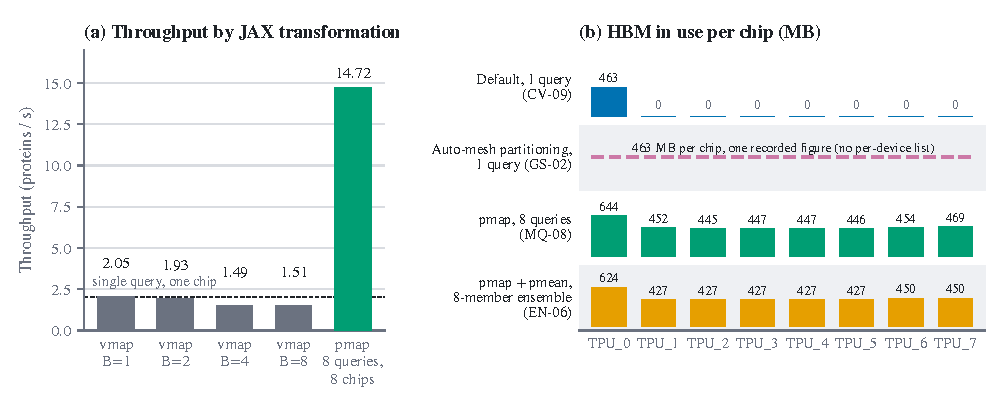
\includegraphics[width=\linewidth]{parallelism_chips.pdf}
  \caption{What each JAX transformation does with the eight-chip slice.
  (a) Steady-state throughput on one chip with \texttt{jax.vmap} at
  batch sizes 1--8, and with \texttt{jax.pmap} mapping eight independent
  queries onto eight chips; the dashed line is the \texttt{vmap}
  batch-size-1 rate (2.051 proteins/second), not the 2.128
  proteins/second single-query baseline behind the 6.92$\times$ figure
  in the text, which comes from a different input family and timer.
  (b) HBM in use on each chip after the second call. Under the default
  path only one chip holds data; the auto-mesh summary reports 463\,MB
  per chip, consistent with replication, stored as a single scalar,
  with no per-device list, and drawn as a dashed line;
  \texttt{pmap} and the \texttt{pmap}+\texttt{pmean} ensemble
  distribute across all eight.
  Row labels give the results-catalogue row IDs.}
  \label{fig:par-chips}
\end{figure}

\subsection{Default execution leaves most of the slice idle}
\label{sec:par-default}

A Cloud TPU~v5e slice with eight chips exposes eight independent
devices to JAX, but nothing about calling \texttt{jax.jit} or invoking
AlphaFold2's own inference function causes computation to spread across
them. Under the default call path, only the first device (\texttt{TPU\_0})
allocates HBM for the model's parameters and activations; the
remaining seven report zero bytes used for the duration of the run.
The rest of the section covers two ways of asking JAX to use the other
seven, one that does not work and one that does, an automatic mechanism
that does not split the model either, and an ensemble built outside
the model.
Figure~\ref{fig:par-chips} summarizes all four cases.

\subsection{Batching within one device: \texttt{jax.vmap}}
\label{sec:par-vmap}

The first attempt batches queries with \texttt{jax.vmap}, which maps a
function over a leading array axis by tracing it once and vectorizing
the resulting operations. This is a within-device transformation: it
changes the shape of the computation that runs on a single core, not
the number of cores it runs on. Applied to AlphaFold2's forward pass, it
does not shard the batch axis across the slice. The sweep records only
\texttt{TPU\_0}'s HBM, which grows with batch size from 487\,MB to
821\,MB. The run write-up reports the other seven chips at 0\,MB, but no
per-device record was retained.

The throughput data confirms this is not a partial win. At batch sizes
1, 2, 4, and 8 the measured throughput is 2.051, 1.928, 1.487, and
1.508 proteins/second, i.e. 0.94$\times$, 0.73$\times$, and
0.74$\times$ the batch-size-1 rate.
No tested batch size exceeds the batch-size-1 throughput, and the
degradation is not monotonic: the batch-8 rate is marginally higher
than batch-4. We report the values as measured rather than fitting a
smooth trend to them. At every batch size tested, vectorization within
a device gives Cloud TPU~v5e no more throughput than not batching at
all.

\subsection{Explicit device mapping: \texttt{jax.pmap}}
\label{sec:par-pmap}

\texttt{jax.pmap} traces the function once and executes one copy per
device, communicating explicitly rather than relying on an
automatic partitioner. Assigning eight independent protein queries to
the eight chips, one query per chip, yields
14.718~proteins/second against a 2.128~proteins/second single-query,
single-chip baseline (0.47\,s per query): a 6.92$\times$ throughput
gain.
Distinct per-chip HBM allocations confirm the work is distributed
across the chips: 644\,MB on
\texttt{TPU\_0} and 445--469\,MB on the remaining seven chips.
On a like-for-like eight-versus-one-chip comparison at a fixed input
length of 100 residues, the corresponding speedup is 6.53$\times$,
that is 81.6\% parallel efficiency; the 118-residue multi-query run's
6.92$\times$ corresponds to 86.5\%.
The two figures answer different questions: 6.92$\times$ is the
throughput gain over a single query on a single chip, and 6.53$\times$
is the eight-over-one-chip speedup on a matched workload,
corresponding to 81.6\% parallel efficiency. Neither should be quoted
in place of the other.

The difference between Section~\ref{sec:par-vmap} and this section is one of
semantics, not tuning. \texttt{vmap} vectorizes an axis
\emph{within} a computation; on its own, with unsharded inputs as
here, it gives the partitioner no reason to place slices of that axis
on different devices. \texttt{pmap} does exactly that: it is, by construction, a
per-device dispatch.

\subsection{Automatic sharding}
\label{sec:par-gspmd}

Between manual \texttt{pmap} and no parallelism at all sits JAX's
automatic partitioner, which infers a sharding of a computation graph
from the sharding of its inputs and outputs without requiring the
programmer to rewrite the function. Two implementations of that idea
exist: GSPMD \citep{xu2021gspmd}, long the default, and Shardy
\citep{shardy2026}, which has since replaced it as JAX's default. The
committed Job configuration pins \texttt{jax[tpu]==0.10.2} and sets no
partitioner flag; that release defaults to Shardy. No retained
execution artifact records the effective setting, so we describe the
automatic-mesh experiment without attributing its outcome to a
confirmed implementation. Both implementations propagate shardings
outward from annotations, which is the property the observation below
turns on, though shared principles do not guarantee identical
decisions on a given graph.
Running AlphaFold2's forward pass under automatic mesh assignment
shows no sign of a sharded model: both retained run summaries record
463\,MB of HBM per chip, equal to the unsharded single-chip footprint,
with steady states of 0.472\,s and 0.473\,s. Each summary stores that
one per-chip figure, with no per-device list, and no compiled
layout or partitioner decision was retained.
That is consistent with replication and gives no evidence of any
reduction in per-chip footprint. It does not by itself establish that
every chip executed an identical full computation.

An earlier account of this result attributed the failure to AlphaFold2's
ensembling, implemented as a sequential \texttt{hk.while\_loop} with no
axis for the partitioner to distribute over. That explanation does not
hold for this experiment: the run in question used
\texttt{num\_ensemble\,=\,1}. AlphaFold2 computes the first ensemble
member outside the loop and enters \texttt{hk.while\_loop} at index~1
with the condition $i <$ \texttt{num\_ensemble}, so during inference
at a single member the loop body never executes (initialization
invokes it once, separately), and it cannot be the cause of the
single-chip-sized footprint the run records. AlphaFold2's released evaluation configuration in fact sets
\texttt{num\_ensemble\,=\,1} by default; the model does not run an
ensemble unless explicitly configured to.

The explanation we find most plausible does not depend on control
flow at all, and we state it as a hypothesis rather than a
demonstrated cause. An automatic partitioner of this kind works by
propagating sharding information outward from whatever annotations
exist on a computation's inputs and parameters. Inspecting AlphaFold2's
Haiku modules and our driver, we find no partition spec attached to
any weight or activation, and none supplied from outside through
input or output shardings. A partitioner given nothing to propagate
has no basis for a split, and replicating the whole computation is
its documented fallback \citep{xu2021gspmd}. DrJAX reports, by
analogy, that removing explicit sharding structure from a
partitioner-based system removes its ability to scale even for
embarrassingly parallel patterns \citep{drjax2024}. Our records do not
contain the evidence that would confirm this account for this graph:
no compiler trace, no retained array layouts, and no ablation that
adds annotations and observes a change. We present the missing
annotations as the likely explanation, consistent with the design
literature and with what we observed, not as a result we measured.

The sequential \texttt{hk.while\_loop} used for AlphaFold2's ensembling
does matter for the external ensemble of Section~\ref{sec:par-fix}:
because the ensemble average is computed inside
a loop with no vectorizable or shardable axis, distributing it
requires an approach that does not depend on the partitioner inferring structure
that the loop does not expose.

\subsection{An external ensemble with \texttt{pmap} + \texttt{lax.pmean}}
\label{sec:par-fix}

Rather than modify AlphaFold2's sequential loop, we sidestep it and build
an ensemble outside the model. The configuration keeps
\texttt{num\_ensemble\,=\,1}, so each chip runs exactly the
single-member forward pass AlphaFold2 always runs; what varies across
chips is the featurization, built eight times with a different
\texttt{random\_seed} each. An explicit \texttt{pmap} places one member
per chip and a \texttt{jax.lax.pmean} averages the resulting
\texttt{predicted\_lddt} logits across devices.
Listing~\ref{lst:fix} contrasts the two shapes.

This demonstration has two limits. AlphaFold2's own ensembling is not
replaced or exercised here: it stays
at a single member throughout, and the loop we describe above never
executes its body, so this experiment shows that \emph{an}
ensemble can be distributed across the slice, not that AlphaFold2's
internal one can. The quantity averaged also differs: AlphaFold2 combines
representations inside the model, whereas \texttt{pmean} here reduces
the per-member confidence logits after the forward pass, which is
where a plain JAX array is available to a collective. The eight members
share one trivial single-sequence MSA and differ only by seed, so they
are near-identical inputs; the result demonstrates the mechanism, not a
scientifically meaningful ensemble.

\noindent\begin{minipage}{\linewidth}
\begin{lstlisting}[caption={AlphaFold2's internal ensembling, which stays at a single member here, against the external ensemble we distribute instead. The per-member forward pass is the same in both.}, label={lst:fix}, language=Python]
# AlphaFold2's own ensembling: the first member is computed outside
# the loop, and hk.while_loop accumulates the rest sequentially on one
# device. We leave this untouched at num_ensemble = 1, so the loop body
# never executes.
representations = evoformer(slice_batch(0))

def body(x):
    i, current = x
    return i + 1, current + evoformer(slice_batch(i))

_, total = hk.while_loop(lambda x: x[0] < num_ensemble, body,
                         (1, representations))

# What we run instead: one differently seeded featurization per chip,
# each a standard single-member forward pass, averaged across devices.
per_member_features = [featurize(query, random_seed=i)
                       for i in range(n_chips)]

@functools.partial(jax.pmap, axis_name="ensemble")
def sharded_apply(feat):
    out = runner.apply(params, rng, feat)
    return jax.lax.pmean(out["predicted_lddt"]["logits"],
                         axis_name="ensemble")

averaged = sharded_apply(stack(per_member_features))
\end{lstlisting}
\end{minipage}

This places the work on the whole slice: all eight chips report nonzero
HBM allocation, and an \texttt{allclose} check on the first and last
returned replicas passes.
The change touches none of AlphaFold2's own modules; only the entry point
that drives ensemble members is replaced. \texttt{jax.lax.pmean}
averages the \texttt{predicted\_lddt} logits emitted by each member;
individual predicted structures are not themselves averaged.
Steady-state latency for the eight-way ensemble-sharded configuration
is 0.538\,s.
No sequential \texttt{num\_ensemble=8} baseline exists in the data, so
no speedup figure is reported or derived for this configuration; it
should not be described as faster or slower than a sequential
ensemble we did not measure.

This result is distinct from Section~\ref{sec:par-pmap}'s multi-query
experiment, which maps eight \emph{independent} protein queries onto
eight chips and measures throughput. Here the eight \emph{members of
one query's ensemble} are mapped onto eight chips, and the question is
whether the reduction that combines them can be executed without a
sequential loop. Both use \texttt{pmap}, but they parallelize different
axes of the problem.

\subsection{Summary}
\label{sec:par-summary}

The slice's eight chips are never disabled or defective. Every
experiment in this section runs on the same hardware. What changes
across the section is how much of that hardware the program
uses: one chip under the default path and under \texttt{vmap},
eight chips under \texttt{pmap} for independent queries, with a
6.92$\times$ throughput gain over a single query at 118 residues and a
6.53$\times$ eight-over-one-chip speedup at 100 residues, one chip's
worth of computation
apparently replicated eight times under automatic sharding, and
eight chips each running a full forward pass once an ensemble is built
outside the model and mapped across them with an explicit
\texttt{pmap}+\texttt{pmean} reduction. The last case distributes
independent members and reduces their confidence logits; it does not
partition one model instance, and does not repair the automatic
sharding of the case before it. In all four cases the hardware is the
same, and the outcome depends on the JAX transformation used to
express the work.


\section{Scaling with Chip Count and Sequence Length}\label{sec:scaling}

\subsection{Measurement grid}
\label{sec:scaling-grid}

We measure throughput of the multi-query \texttt{pmap} configuration
from Section~\ref{sec:parallelism} on a full grid of chip count
(1, 2, 4, 8) and sequence length (100, 250, 500, 1000 residues), 16
points total, each a single steady-state measurement with no
repeat.
At chips=8, throughput falls from 19.153 to 0.522 proteins/second as
length grows from 100 to 1000 residues. At length=100, it rises from
2.935 to 19.153 proteins/second as chips grow from 1 to 8. Every point
on this grid uses the rotated-alphabet input described in
Section~\ref{sec:methodology}, not the 118-residue toy sequence used
for the single-query experiments elsewhere in the paper. Because chip
count and length are varied on the same input family and the same
timer, this grid is the paper's cleanest measure of what adding chips
buys.

\begin{figure}[H]
  \centering
  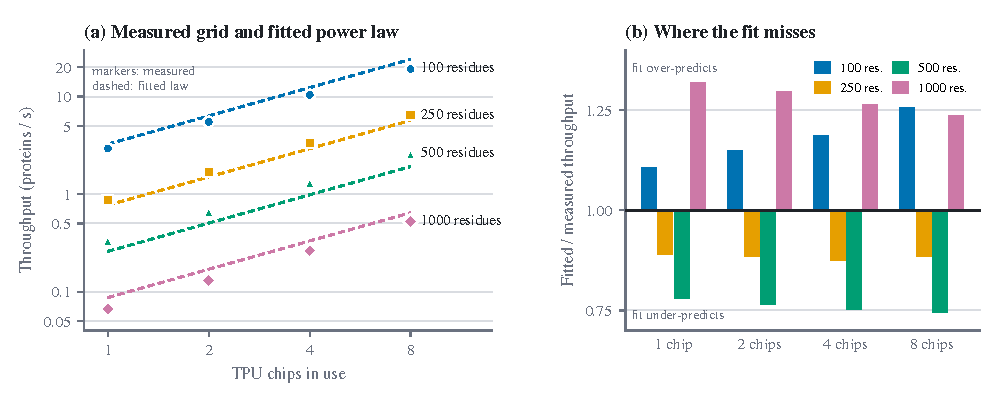
\includegraphics[width=\linewidth]{scaling_grid.pdf}
  \caption{The 16-point scaling grid (multi-query \texttt{pmap},
  repeated-alphabet inputs, one process per point). (a) Measured
  throughput against chips in use for each sequence length, with the
  fitted law $4527.77 \times \mathrm{chips}^{0.963} \times
  \mathrm{length}^{-1.572}$ drawn dashed. (b) Fitted divided by measured
  throughput at every grid point: the fit over-predicts at 100 and 1000
  residues and under-predicts at 250 and 500, a systematic pattern. The one-chip point at 1000 residues is recorded
  to two significant figures.}
  \label{fig:scaling-grid}
\end{figure}

\subsection{Measured speedup at each length}
\label{sec:scaling-speedup}

The eight-over-one-chip speedup
is 6.53$\times$ at length 100, rising to 7.47$\times$ at 250,
7.76$\times$ at 500, and 7.91$\times$ at 1000.
The four-over-one and two-over-one speedups show the same pattern:
3.55$\times$ to 3.97$\times$, and 1.88$\times$ to 1.98$\times$,
respectively, moving toward their ideal values (4$\times$, 2$\times$)
as length grows.
Scaling efficiency is worst at the shortest sequence length in this
grid, which is also closest to the 118-residue input used
throughout the rest of the paper: the fixed per-call overhead that
Sections~\ref{sec:profiling} and~\ref{sec:parallelism} describe
makes up a larger share of a short call, leaving less of the
eight-chip speedup to be realized. At longer sequences, where
per-chip compute dominates more of the call, the measured speedup
approaches ideal linear scaling.

\subsection{A descriptive power-law fit}
\label{sec:scaling-fit}

An ordinary-least-squares fit in log-log space summarizes the grid as
\begin{equation}
  \text{throughput} \approx 4527.77 \times \text{chips}^{0.963} \times \text{length}^{-1.572},
  \quad R^2 = 0.981.
  \label{eq:scaling-fit}
\end{equation}
The chip exponent, 0.963, is close enough to 1 to describe scaling
across chips as near-linear over this range. The length exponent,
$-1.572$, is steeper than $-1$: throughput falls faster than simple
inverse proportionality with sequence length, consistent with the
pair representation's cost growing faster than linearly in residue
count (Section~\ref{sec:background}).

$R^2 = 0.981$ describes the fit in log space across all 16 points; it
does not mean the fit tracks the grid closely at any one length.
The ratio of fitted to measured throughput follows a systematic
pattern: the fit over-predicts
by 10--26\% at length 100 and by 23--32\% at length 1000, and
under-predicts by 11--13\% at length 250 and by 22--26\% at length
500 (Figure~\ref{fig:scaling-grid}).
A single global exponent therefore approximates a relationship that
curves, and we use the fit only as a summary of this grid. We give
per-length residuals instead of a regression interval on the
exponents: with one measurement per cell the deviation is dominated by
misspecification, not by sampling noise, and an interval would
understate it. A chip exponent close to 1 predicts that cost per
prediction is roughly flat in chip count. Section~\ref{sec:cost} tests
this on the measured grid and finds it holds only at longer
sequences.



\section{Cost Analysis}\label{sec:cost}

\subsection{Pricing basis}
\label{sec:cost-basis}

We price each backend at an August 2026 on-demand rate, and the three
rates do not come from the same place. The TPU figure, \$1.20 per
v5e chip-hour, so \$9.60/hour for an 8-chip pod, is Google Cloud's own
published price \citep{googletpupricing}. The GPU figure,
approximately \$0.35/hour for an NVIDIA T4 instance, is taken from a
third-party survey of Google Cloud prices carried out in the same
month. The CPU figure, approximately \$0.19/hour for an instance
comparable to \texttt{n2-standard-4}, is our own estimate, for which we
recorded no dated source. It is the weakest input here, and we use it
only for the CPU row. The catalogue marks all three as input
assumptions, not measurements. These are list prices
for a hypothetical always-on rental, not the cost we were actually
billed: our TPU cluster was a Stanford course allocation, and our
Colab CPU/GPU sessions ran on shared, non-dedicated infrastructure.
We could not obtain a smaller TPU slice than the full 8-chip pod on
our GKE setup, so the single-call TPU cost below bills for the whole
pod even though only one chip does work. The chip-count analysis in
Section~\ref{sec:cost-scaling} instead prices slices of 1, 2, 4 and 8
chips at the same per-chip rate, which prices \emph{hypothetical}
slices: 2- and 4-chip subsets failed to initialize on our setup with a
libtpu topology error, so no smaller slice was ever billed.
The \$1.20 rate was still listed unchanged when we re-checked Google's
pricing page on 2026-09-17.

\subsection{Cost per prediction, single call}
\label{sec:cost-baseline}

Combining these rates with the steady-state throughput measured in
Section~\ref{sec:results-hardware} gives the per-backend cost of 1{,}000
predictions in Table~\ref{tab:cost-baseline}.

\begin{table}[H]
\centering\small
\caption{Cost per 1{,}000 single-call predictions at on-demand list
prices, from August steady-state throughput. The TPU row bills the full
8-chip pod.}
\label{tab:cost-baseline}
\begin{tabular}{lrr}
\toprule
Backend & Throughput (pred/h) & \$ / 1{,}000 predictions \\
\midrule
CPU                          & 17.0   & \$11.19 \\
GPU (T4)                     & 275    & \$1.27  \\
TPU pod, 1 of 8 chips active & 7{,}660 & \$1.25  \\
\bottomrule
\end{tabular}
\end{table}

The TPU pod and the GPU land at almost the same \$/1k despite the pod
costing 27.4$\times$ more per hour: the chip is far faster than the
GPU, 7{,}660 against 275 predictions per hour, but on this single-chip
workload the pod bills for seven idle chips (87.5\% of the pod, the
same idle-chip finding as Section~\ref{sec:parallelism}), and the two
effects very nearly cancel. If it were possible to rent
one TPU chip alone at the same per-chip rate, the hypothetical cost
would be \$0.157/1k, about 8.1$\times$ cheaper than the GPU. That
makes the pod-billing effect, not the chip's own economics, the reason
the \$1.25 figure looks unremarkable next to the GPU. The near-equality is specific to the August GPU baseline: on the
September rerun the GPU would sit near \$0.64/1k and the pod would be
about twice as expensive (Section~\ref{sec:rh-variability}). The
idle-chip mechanism does not depend on which baseline is used.


Renting the whole pod stops being wasteful once all 8 chips do useful
work. Using the multi-query \texttt{pmap} throughput from
Section~\ref{sec:parallelism} (6.92$\times$ over one chip, 14.718
proteins/second across 8 independent proteins) at the same \$9.60/hour pod
rate gives
$
\$9.60 \,/\, (14.718 \times 3600) \times 1000 \approx \$0.181\text{/1k predictions},
$
within about 15\% of the single-chip hypothetical rate once the pod is
kept busy. The two rates are not strictly commensurable: the
multi-query throughput comes from the rotated-alphabet input family
timed around \texttt{apply}, while the single-chip baseline folds the
fixed synthetic sequence and times \texttt{predict}, which also
includes AlphaFold2's host-side confidence metrics
(Section~\ref{sec:meth-workload}). The like-for-like chip-count
comparison is the 100-residue grid of Section~\ref{sec:cost-scaling}.

\subsection{Cost as a function of chip count}
\label{sec:cost-scaling}

Section~\ref{sec:scaling} finds throughput scaling as
$\mathrm{chips}^{0.963}$, just below linear, which by itself would
predict that cost per prediction is nearly independent of chip count.
We test this directly on the measured chip-count $\times$ sequence-length
grid, not on the fitted formula, in Table~\ref{tab:cost-scaling}. Each
point is the multi-query \texttt{pmap} workload, and each cost charges
only the chips in use (chips $\times$ \$1.20 per hour divided by
measured throughput). This prices a \emph{hypothetical} slice of that
size at the same per-chip rate, unlike Table~\ref{tab:cost-baseline},
which bills the whole 8-chip pod; as Section~\ref{sec:cost-basis}
notes, slices smaller than eight chips could not be obtained on our
setup.

\begin{table}[H]
\centering\small
\caption{Cost per 1{,}000 predictions by chip count and sequence length,
computed from measured throughput on the scaling grid. The last column
is the increase from 1 to 8 chips.}
\label{tab:cost-scaling}
\begin{tabular}{lrrrrr}
\toprule
Length (residues) & 1 chip & 2 chips & 4 chips & 8 chips & 1$\to$8 \\
\midrule
100  & \$0.114 & \$0.121 & \$0.128 & \$0.139 & +23\% \\
250  & \$0.386 & \$0.394 & \$0.399 & \$0.413 & +7\% \\
500  & \$1.004 & \$1.012 & \$1.019 & \$1.036 & +3\% \\
1000 & \$5.051 & \$5.089 & \$5.089 & \$5.109 & +1\% \\
\bottomrule
\end{tabular}
\end{table}

Adding chips is not free: going from 1 to 8 chips raises cost per
prediction by 22.6\% at 100 residues (23\% in the table's integer
rounding, computed from the unrounded throughputs). The penalty shrinks quickly with
sequence length, to 7\% at 250, 3\% at 500 and about 1\% at 1000
residues; the last figure is within the rounding of the one-chip
throughput at that length, which the grid records to only two
significant figures. On this grid, with one run per point, the
near-invariance implied by the fitted exponent therefore holds only for
long sequences. For short sequences, close to
the 118-residue input of our single-query experiments, using more chips
has a real, double-digit cost.

\subsection{Practical implication}
\label{sec:cost-implication}

Chip count should therefore be chosen for latency and throughput
requirements, not to minimize unit cost: the cost penalty for using
more chips is modest, but it is not zero, and it is largest exactly in
the short-sequence regime this study otherwise focuses on. In our
measurements, the dominant cost lever for this workload is not how
many chips are rented but whether they are kept busy. Renting an
8-chip pod
to run a single-chip job wastes 87.5\% of what is being paid for; the
same pod running eight independent proteins in parallel does not cost
more per hour and delivers 6.92$\times$ the predictions, an 86.5\%
parallel efficiency.

All figures in this section use a single steady-state measurement per
backend (Section~\ref{sec:limitations}). We did not recompute the CPU
figures against the September sessions: no session has a better claim
than another to being the reference
(Section~\ref{sec:rh-variability}).


\section{Portability to AlphaFold3}\label{sec:alphafold3}

We treat AlphaFold3 not as a second benchmark study but as a portability
question: does what Section~\ref{sec:parallelism} and
Section~\ref{sec:results-hardware} found about AlphaFold2 on TPU
generalize to a newer model in the same family. AlphaFold3 is run with
its real, trained weights, not the untrained weights used for AlphaFold2
elsewhere in this paper (Section~\ref{sec:methodology}). The setup,
timings and per-sample score comparisons are in
Appendix~\ref{app:af3}; two findings bear on the argument of this
paper.

\subsection{No TPU backend in the release we tested}
\label{sec:af3-tpu}

Running the same TPU Job configuration used throughout this paper
against AlphaFold3 fails immediately: \texttt{run\_alphafold.py} rejects
\texttt{-{}-jax\_backend=tpu} at flag parsing, after 5.588\,s, before any
model code executes. The accepted values are \texttt{cpu}, \texttt{gpu}
and \texttt{mps}.
This matches AlphaFold3's own documentation, which lists CPU or an
NVIDIA GPU of compute capability 7.0 or greater as the supported
targets \citep{af3docs2026}. TPU is not a documented target. The
rejection above is a Job failure on our own cluster, not an inference
from the documentation alone.


\subsection{Output differs across backends}
\label{sec:af3-body-repro}

Running the identical seed and input on the same backend but different
machines (Stanford's CPU cluster versus the Colab CPU) changes the
per-sample ranking score by at most 1.67\%, and by under 0.1\% on four
of five samples; running it on different backends (Colab CPU versus
Colab GPU) changes it by up to 32.33\% on one sample.
The across-backend divergence is roughly an order of magnitude larger
than the across-machine, same-backend noise. A plausible, documented
cause exists in AlphaFold3's own performance notes, which report known
numerical issues on CUDA Capability 7.x devices such as the Colab T4
\citep{af3docs2026}. We did not isolate the operation responsible, so
this cause remains plausible and unconfirmed
(Appendix~\ref{app:af3-repro}).

\subsection{Summary}
\label{sec:af3-summary}

Section~\ref{sec:parallelism}'s central finding, that realized
performance on TPU depends on how parallelism is expressed rather than
on the accelerator alone, cannot be tested on AlphaFold3 at all: the
release we tested has no TPU path to express parallelism on in the
first place. The broader caution of this paper does carry over: a
newer model in the same family changes not just speed but which
backends are available at all, and, on a documented edge case of GPU
hardware, how far the reported output can be trusted to match across
sessions.


\section{Related Work}\label{sec:related-work}

\subsection{AlphaFold2 acceleration}
\label{sec:rw-alphafold}

AlphaFold2 inference optimization has been studied almost entirely on
NVIDIA GPUs. ParaFold separates the CPU-bound MSA search stage from
GPU inference and avoids redundant JAX recompilation across a batch of
proteins by sorting them by length, reporting an average 13.8$\times$
speedup over baseline AlphaFold2 \citep{zhong2022parafold}. FastFold
introduces Dynamic Axial Parallelism, a model-parallel scheme specific
to AlphaFold2's Evoformer, together with an activation-memory reduction
technique (AutoChunk); its arXiv version reports scaling to 512 GPUs
\citep{cheng2022fastfoldarxiv}. We do not place our 86.5\% parallel
efficiency on 8 chips (Section~\ref{sec:parallelism}) next to the
efficiency reported there: that figure is a \emph{training} scaling
result and ours is inference throughput, and the two are not directly
comparable \citep{cheng2024fastfold,cheng2022fastfoldarxiv}. APACE distributes
AlphaFold2's ensemble across hundreds of A100 GPUs to reduce
time-to-solution on real structures from weeks to minutes
\citep{apace2024}. ScaleFold and HelixFold scale AlphaFold2
\emph{training}, rather than inference, to large GPU clusters
\citep{scalefold2024,helixfold2022}. Uni-Fold reimplements AlphaFold2 in
PyTorch specifically because the original was TPU-trained and TPU
access is scarce, an explicit statement of the accessibility gap this
paper's TPU results speak to \citep{unifold}. OpenFold is a widely used GPU-targeted
reimplementation and ColabFold a widely used inference workflow around
the released models; ColabFold's roughly
90$\times$ batch speedup, achieved in part by avoiding recompilation
across a batch, is the same JAX-recompilation cost that
Section~\ref{sec:profiling}'s retained trace analysis reports at the
function level on a different accelerator \citep{openfold2024,colabfold2022}.
AlphaFold2 optimization has thus been a GPU-and-CPU-centric
literature; none of it reports TPU experiments.

Two works come closer to the TPU setting considered here, but address
different questions. ManyFold is a JAX library for
training and validating protein-folding models that does run on TPU,
but the TPU role there is training a different, smaller model
(pLMFold) on a TPU v2-128 pod; its own AlphaFold-style inference-speed
comparison runs on a GPU, not a multi-chip TPU slice
\citep{villegas-morcillo2023manyfold}. MatrixFold describes itself as
the first systematic study of AlphaFold2 mixed-precision inference
\emph{on a many-core ARM CPU architecture}; the framing is close to
this paper's, but the hardware is not
\citep{matrixfold2026}. Neither measures AlphaFold2 inference across a
multi-chip TPU slice using \texttt{pmap}, \texttt{vmap}, or automatic
partitioning, which
is this paper's subject.

JAXBench includes operators extracted from AlphaFold2 among the TPU
kernels it benchmarks \citep{jaxbench2026}; it benchmarks kernels, not
the end-to-end model. A recent characterization of AlphaFold3 profiles
that model's bottlenecks on CPUs and GPUs \citep{iiswc2025af3} and does
not include TPU.

\subsection{Accelerator benchmarking methodology}
\label{sec:rw-benchmarking}

Outside the AlphaFold family, recent trace-based and end-to-end
comparisons of TPU against GPU on language models
\citep{ding2026cclbench,gemma2026tpu} are precedent for comparing the
two through platform-specific stacks on the same model and task; none
touches protein folding, and we do not draw on their results.
Jouppi et al.'s original and TPU v4 architecture papers
\citep{jouppi2017tpu,jouppi2023tpuv4}, together with Google's own v5e
documentation \citep{googletpuv5e}, are our source for the hardware
specifications in Section~\ref{sec:background}, since the v5e
generation used throughout this paper has no dedicated peer-reviewed
architecture paper of its own.

\subsection{Compilation and parallelism frameworks}
\label{sec:rw-frameworks}

GSPMD, the design JAX/XLA's automatic partitioners follow, shards a
computation by propagating sharding decisions outward from explicit
annotations, and its own presentation treats a computation carrying
none as a limiting case of that design rather than as a failure
\citep{xu2021gspmd}. DrJAX documents a
closely related case: removing explicit sharding structure from a
partitioner-based MapReduce system removes its ability to scale efficiently,
even for an embarrassingly parallel pattern \citep{drjax2024}. This is
the closest published precedent to Section~\ref{sec:parallelism}'s
observation, and to our hypothesis that AlphaFold2's unannotated Haiku
modules leave the partitioner nothing to shard on. Neither paper
reports this on AlphaFold2 or on any protein-folding model. We present
our result as consistent with what that design implies when
annotations are absent, not as a new mechanism or a confirmed one. Recent JAX/XLA
measurements on TPU v6e report first-call compilation costs of the
same order as ours \citep{jitcompile2026}, and a separate benchmark
confirms that a new input shape retriggers the cost
\citep{warmup2025}. Finally, Duet Benchmarking and the SPEC
Research Group's methodology for reproducible cloud performance
evaluation document that same-type cloud instances can vary
substantially in measured performance due to hardware heterogeneity
the provider does not expose to the tenant
\citep{bulej2020duet,papadopoulos2021specrg}; we read the gaps
Section~\ref{sec:rh-variability} reports as consistent with that
literature, without a cause isolated, and not as an independent
confirmation of it on ML accelerators.


\section{Discussion}\label{sec:discussion}

The results in this paper separate two things that are easy to
conflate when picking an accelerator: what the hardware is capable of,
and what a given program actually gets from it. On every measure we
took, the single v5e chip's raw capability was never in question. What
varied, sometimes by an order of magnitude, was how much of that
capability the default execution path exposed, and closing that gap
required knowing which JAX transformation to reach for
(Section~\ref{sec:parallelism}), understanding what a profiler trace
was and was not measuring (Section~\ref{sec:profiling}), and pricing a
slice by whether it was kept busy rather than by its hourly rate
(Section~\ref{sec:cost}). None of this required modifying AlphaFold2's
own source.

\subsection{Steady state versus cold start}
\label{sec:disc-when}

The single-chip comparison in Section~\ref{sec:results-hardware}
favors the TPU by a wide margin at steady state, but the same section
shows a raw 59.1$\times$ gap between the TPU's cold and steady-state
call, uncorrected because no TPU profiler-overhead log survives to
correct it. Whatever the true corrected value, the qualitative point
carries: a workload dominated by one-off calls at varying input shapes
pays the compilation cost on nearly every call, while a workload that
reuses one compiled shape repeatedly, such as sustained serving of a
fixed-length input, amortizes it away. This paper measures a
steady-state advantage, and nothing here tests whether it holds for a
workload that never reaches steady state.

\subsection{The cost of the default path}
\label{sec:disc-default}

A user who runs our unmodified single-query forward-pass driver on an
8-chip TPU slice gets the result Section~\ref{sec:parallelism}
describes: one chip working, seven idle, with no error or warning that
anything is wrong. We did not test every production entry point, but
nothing in AlphaFold2's default configuration asks for anything
different. Section~\ref{sec:cost}
shows what this costs in money as well as in throughput: the pod bills
for 87.5\% capacity that produced no output. No bug is involved:
on our reading of the evidence, this is the documented behavior of
\texttt{jax.jit} and of an automatic partitioner given a model with no
sharding annotations. The gap this paper
measures is therefore not primarily a hardware limitation or a flaw in
AlphaFold2's implementation, but a gap in what a user needs to know
about JAX's parallelism primitives before an 8-chip rental delivers
8 chips of work.


\section{Limitations}\label{sec:limitations}

\textbf{One sequence length for most experiments.} Every single-query
timing in Sections~\ref{sec:results-hardware} and
\ref{sec:profiling} uses one 118-residue sequence. The
sequence-length sweep behind Section~\ref{sec:scaling}'s fit covers
100 to 1000 residues, but on a different, rotated-alphabet input
family (Section~\ref{sec:methodology}) that we do not compare
timings against the 118-residue results.

\textbf{One TPU generation.} All TPU measurements use v5e; we have no
data on v6e, v7 (Ironwood), or the announced TPU 8t/8i generation
\citep{googletpuv8ann2026}, and make no claim about whether any
finding here holds on a different generation.

\textbf{Untrained weights.} AlphaFold2 runs with randomly initialized
parameters throughout (Section~\ref{sec:methodology}). This is
deliberate for a timing study and does not affect the compiled
graph's shape, but it means every result here is a statement about
compute, not about prediction quality, and we did not measure whether
timing with trained weights is the same.

\textbf{Asymmetric isolation.} The TPU ran as a dedicated Kubernetes
Job. CPU and GPU ran on shared Colab runtimes whose underlying
machine the provider chooses and can change between sessions
(Section~\ref{sec:rh-variability}). The session-to-session
variability we measured and report is therefore a property of the
CPU/GPU setup specifically, not evidence about TPU stability one way
or the other.

\textbf{The headline speedups are computed from baselines that did not
reproduce.} The 27.8$\times$ TPU-over-GPU figure divides the August GPU
steady state by the TPU one, and the 451$\times$ TPU-over-CPU figure
divides the August CPU steady state by it; both numerators moved on
rerun, the GPU one by roughly a factor of two and the CPU one by
1.6--1.7$\times$, gaps we could not explain
(Section~\ref{sec:rh-variability}). We keep the August figures because
they come from the same measurement campaign as the TPU numbers and no
TPU rerun exists to pair with the September values: substituting them
would compare across sessions in exactly the way this section's own
finding argues against. Our records do not, however, establish that the
three August backends ran in a single session: the result files carry
no timestamp or session identifier, archived notebook output dates the
CPU and GPU runs to 2026-08-08, and the TPU run is dated only by its
commit (Section~\ref{sec:meth-provenance}).
The consequence is that these ratios compare one chip against one T4
and two vCPUs respectively, on one measurement campaign whose baselines
later moved, and should not be read as portable hardware constants.

\textbf{Most TPU measurements are single runs.} Two exceptions: a
three-repeat check on the single-query configuration (coefficient of
variation under 1.2\% on every timed region), and the auto-mesh
experiment, which ran twice. Neither extends to the multi-chip
\texttt{pmap} or scaling-grid experiments. Access to the
TPU cluster ended with the course that provided it, so none of this
can be regenerated or repeated.

\textbf{Provenance gaps predating this project's audit.} The original
August baselines were produced by scripts that were never committed
to version control in the form that ran (Section~\ref{sec:methodology}),
so those specific numbers cannot be reproduced bit-for-bit from the
released repository. The September reruns close this gap for CPU and
GPU only. Several supporting figures, including the raw XLA profiler
trace behind Section~\ref{sec:profiling}, the vendor hardware
specifications in Section~\ref{sec:background}, and one AlphaFold3
Stanford-CPU timing, come from project documentation, with no raw data
file behind them in the repository.

\textbf{The measured software stack is only partly pinned.} On the TPU
Jobs only \texttt{jax[tpu]} was pinned, to 0.10.2;
\texttt{dm-haiku}, \texttt{tensorflow-cpu}, \texttt{numpy},
\texttt{biopython}, \texttt{ml\_collections} and \texttt{absl-py} were
installed unpinned at container start-up, and the AlphaFold2 commit was
not recorded (Section~\ref{sec:meth-software}). Re-running the same
scripts today may therefore resolve a different dependency set from the
one that produced these numbers, and any effect of that difference
cannot be separated from the hardware and session effects discussed
above.

\textbf{Cost figures rest on a single measurement per backend and one
pricing snapshot.} Section~\ref{sec:cost} prices each backend
from one steady-state throughput value, not from the session-level
distributions of Section~\ref{sec:rh-variability}, and uses on-demand
list prices from a single date. Neither changes qualitatively with
small input variation, but neither is a distribution.

\textbf{The scaling-law fit is an approximation, not a tight one.}
Section~\ref{sec:scaling} reports the fitted curve's actual deviation
from the measured grid directly, up to 32\% at the extremes of the
tested length range; with a single measurement per grid cell we do not
compute a confidence interval. A global two-exponent power law is a
convenient summary of this grid, not a precise model of it.

\textbf{AlphaFold3 results are effectively single runs per backend.}
Each of the five diffusion samples in Section~\ref{sec:alphafold3}
comes from one process invocation, not five independent runs, so the
CPU-versus-GPU divergence there is one comparison, not a distribution
of comparisons, and the documented cause we report for it
(Appendix~\ref{app:af3-repro}) is plausible but unconfirmed.


\section{Conclusion and Future Work}\label{sec:conclusion}

On the same AlphaFold2 inference code and the same input, accelerator
choice alone did not determine what a user actually got. A single TPU
v5e chip beat a T4 GPU by 27.8$\times$ at steady state on our August
baseline, a figure Section~\ref{sec:limitations} qualifies. That
number also described one of eight allocated chips; the other seven sat at
0\,MB until we explicitly asked JAX to use them
(Section~\ref{sec:parallelism}), and the pod's list price reflected
all eight regardless (Section~\ref{sec:cost}). Vectorizing with
\texttt{jax.vmap} never recovered them. Mapping independent queries
across devices with \texttt{jax.pmap} did, giving eight chips
6.53--7.91$\times$ the throughput of one on a matched grid. Automatic sharding, meant to make that mapping
unnecessary, left the per-chip footprint at its single-chip size,
consistent with replication. Our best explanation is that AlphaFold2's
Haiku modules carry no sharding annotations for it to propagate from,
which we could not confirm from retained compiler evidence. Separately,
we showed that an ensemble built outside the model can be mapped
across all eight chips with an explicit \texttt{pmap} and
\texttt{jax.lax.pmean} reduction, without changing AlphaFold2's
source. None of this was
visible from steady-state throughput alone. The cold-start cost
appeared only in a profiler trace (Section~\ref{sec:profiling}), the
baseline drift only when we reran the same benchmark weeks later
(Section~\ref{sec:results-hardware}), and the idle-chip cost only when
the slice was priced as it is billed (Section~\ref{sec:cost}).

\subsection*{Future work}

Three extensions follow directly from what this paper could not test.
Google's TPU 8i, announced before these measurements but not evaluated
here \citep{googletpuv8ann2026}, is inference-specialized silicon.
Testing it against the first-call compilation costs characterized here
is a natural next step once it is available.
FastFold's Dynamic Axial Parallelism is a model-parallel alternative
to the data-parallel approach this paper uses. Whether it transfers to
TPU, and how it compares to the \texttt{pmap}-based approach here, is
untested. And the single sequence length and single TPU generation
noted in Section~\ref{sec:limitations} are the most direct gaps to
close: longer sequences, multimer inputs, and later TPU generations
would each test whether the mechanisms identified here, not just the
specific numbers, generalize beyond this study's setup.


\section*{Code and Data Availability}
All benchmark scripts, Kubernetes Job definitions, notebooks, raw result
files and the results catalogue that every number in this paper is taken
from are available at
\url{https://github.com/lorenzopazienza/alphafold-tpu-benchmark}, branch
\texttt{paper}, commit \texttt{a63e955}. The catalogue
(\texttt{paper/data/canonical\_results.md}) gives, for each value, the
file and field it comes from and whether it is measured, derived, an
input assumption or reported only; \texttt{paper/sections/methodology.md} documents the
provenance of the setup line by line, including what our records do not
contain. The reproduction runs of September~2026
(\texttt{results/repro/}) each store the benchmark commit they ran from
together with the resolved package versions and host CPU of their
session. The TPU experiments ran with \texttt{jax[tpu]==0.10.2};
their remaining dependencies were not pinned, as
Section~\ref{sec:limitations} states.

\section*{Acknowledgments}
This work was carried out during the ME344 High Performance Computing
and AI Systems course at Stanford University (Summer Session 2026). We
thank Mourad Bouache (Google), who taught the course, for his guidance
throughout the project and for the opportunity to present this work at
Google, and Steve Jones, Director of the Stanford High
Performance Computing Center and Research Scientist at Stanford
University, for access to the TPU~v5e cluster used throughout. We also
thank the Department of Mechanical Engineering at Stanford University
for hosting the course.

\bibliographystyle{plainnat}
\bibliography{references}

\appendix
\section{AlphaFold3 Setup, Timings and Score Comparison}\label{app:af3}

This appendix records how AlphaFold3 was brought up on each backend,
its timings, and the per-sample score comparisons summarized in
Section~\ref{sec:alphafold3}.

\subsection{Bringing AlphaFold3 up}
\label{app:af3-infra}

AlphaFold3 is a separate, diffusion-based codebase, not a version
increment of AlphaFold2, and required meaningfully more engineering to
run on every backend. Unlike AlphaFold2's pure-Python install,
AlphaFold3 needs a native C++ build step (\texttt{libcifpp} and pybind11
bindings) unavailable without root on our cluster's login node, and a
separate \texttt{build\_data} step that constructs the Chemical Component
Dictionary the model needs at start-up. Skipping it does not fail at
start-up but a few seconds into the run, with a missing-file error. The T4
also required \texttt{XLA\_FLAGS=-{}-xla\_disable\_hlo\_passes=%
custom-kernel-fusion-rewriter}, documented in AlphaFold3's own
Dockerfile comments: without it the run raises a \texttt{ValueError}
before any computation starts. Its
released weights decompress to 1.15\,GB. That is roughly 3.3$\times$ an
AlphaFold2 model, measured against an approximately 350\,MB AlphaFold2
figure taken from our own notes; we did not weigh a checkpoint, since
these runs initialize AlphaFold2 randomly and never load a trained
one.
On our cluster, the C++ build step had to run inside a Kubernetes Job,
for the same reason the rest of this paper's
TPU work does: no root access outside a Job.

\subsection{CPU and GPU results}
\label{sec:af3-cpuresults}

AlphaFold3's own timed model-inference region (one seed, five diffusion
samples, including JIT compilation, since AlphaFold3 makes a single
model call per process with no warm-up) runs 2401.38\,s on the Colab
CPU and 86.21\,s on the Colab T4, a 27.86$\times$ GPU-over-CPU speedup
with compilation included on both sides.
As with AlphaFold2, we do not compute an AlphaFold3-over-AlphaFold2
speed ratio anywhere in this paper: the two models differ in recycling
depth, in whether the timed region includes compilation, and in how
many output samples one call produces, and an early draft of this
comparison that did not control for those differences reached the
wrong sign. We report each model's own internal ratios and nothing that
divides one model's timing by the other's.

\subsection{A reproducibility finding}
\label{app:af3-repro}

Section~\ref{sec:af3-body-repro} gives the headline comparison. Across
backends, the best-ranked sample's score falls from 0.41 to 0.33 and its
fraction of disordered residues from 0.37 to 0.21.
The divergence is not explained by anything in our own methodology: the
two runs share seed, input and AlphaFold3 version. They are not identical in every respect: the GPU
run also sets the XLA flag described above, which the CPU run does not
need, and we did not isolate that flag's effect on the outputs.

A plausible, independently documented cause exists. AlphaFold3's own
performance documentation states that CUDA Capability 7.x devices have
known numerical issues, and recommends a specific XLA flag as a
workaround \citep{af3docs2026}; the Colab T4 used throughout this paper
is compute capability 7.5, inside that range, and the same flag was
required to get any AlphaFold3 result on it at all
(Appendix~\ref{app:af3-infra}). Community reports on AlphaFold3's own
issue tracker corroborate output problems on GPUs below the officially
tested tier (A100 and H100), though we did not find that tracker
discussion naming compute capability 7.5 specifically. We treat the
documented CUDA-capability issue, not the tracker discussion, as the
source for this explanation, and report it as a plausible cause
consistent with our own measurements. It is not confirmed: we did not
instrument AlphaFold3 internally to isolate which operation
produces the divergence.



\end{document}
